%%=============================================================================
%% Methodologie
%%=============================================================================

\chapter{\IfLanguageName{dutch}{proof-of-concept}{proof-of-concept}}%
\label{ch:proof-of-concept}

In dit hoofdstuk wordt de implementatie van de proof-of-concept uiteengezet. Er zal een Space Invaders-spel worden ontwikkeld voor AllPhi, dat zij kunnen gebruiken of repliceren als een interactieve uitdaging tijdens evenementen. 

Het spel zal de vorm aannemen van een eenvoudig videospel waarin de speler diverse basisfunctionaliteiten kan uitvoeren, zoals bewegen, schieten, punten verdienen, enzovoort. Alvorens de implementatie aan te vangen, wordt een visuele representatie van het beoogde spel gecreëerd. Hiervoor dient het originele Space Invaders-spel als referentiekader.

Binnen het spel zullen verschillende typen vijanden aanwezig zijn, evenals bunkers waarachter de speler dekking kan zoeken. Daarnaast zal een willekeurig gegenereerde UFO periodiek aan de linkerkant van het scherm verschijnen, waarna deze zich naar rechts beweegt terwijl er op de speler wordt geschoten. Alle vijanden kunnen worden vernietigd, wat de speler punten oplevert. De hoeveelheid punten die de speler verdient, is afhankelijk van de positie van de vijand binnen de verschillende lagen: hoe hoger de laag, des te meer punten worden toegekend.

\section{Doelstelling}
De proof of concept heeft als doelstelling een space-invaders videospel te implementeren in Unity en Godot met gebruik makend van C\# als de scripttaal voor de engines. Hierdoor weet Allphi of het mogelijk is en zouden ze het kunnen recreëren.

\section{Implementatie in Unity}
\subsection{Installatie van Unity}
Unity heeft hiervoor hun eigen applicatie genaamd Unity Hub. Hierop kan je de versies die Unity aanbiedt raadplegen en installeren op je systeem. De Unity projecten die aanwezig zijn op het systeem herkent de applicatie en voegt deze toe zodat je op een plaats alle nodige zaken kan raadplegen. Het kan zijn dat bij nieuwere versies oude zaken niet meer correct zullen werken. Hiervoor is het aangeraden om bij de start van je project een versie te kiezen en hierbij te blijven.

\subsection{De installatie van unity hub zelf}
Navigeer naar de website van Unity zelf (https://unity.com/download) en klik op de download knop. Dit zal de setup opslaan op je pc. Na het downloaden voer deze uit. Installeer de Unity Hub op de gewenste plaats. Na dat de installatie is voltooid van Unity Hub vraagt deze applicatie waar je de Editor voor Unity wilt installeren. Laat dit op de standaard plaatst staan over verander dit naar de gewenste plaatst. De download en installatie van de Unity Game Engine zal van start gaan. Wacht totdat deze voltooid. Dit kan even duren. 
\begin{figure}[H]
    \centering
    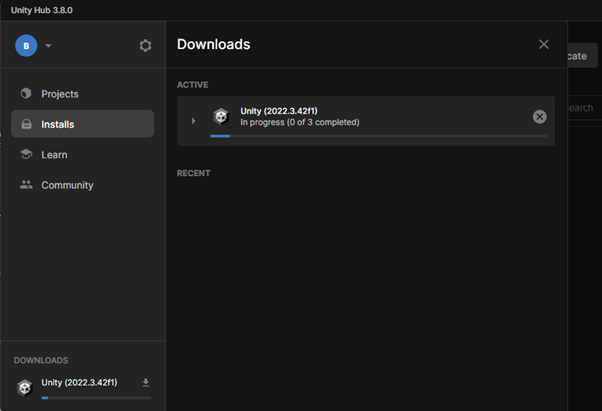
\includegraphics[width=1\textwidth]{UnityHub.png}
    \caption{UnityHub}
    \label{fig:UnityHub}
\end{figure}

Voor de scripts te schrijven voor Unity wordt er gebruik gemaakt van Visual Studio. Visual studio is gratis te verkrijgen op hun website (https://visualstudio.microsoft.com/)

\subsection{Het aanmaken van het project}
Nu de installatie van Unity voltooid kan er een project aangemaakt worden. Dit kan via de knop “New Project” gedaan worden.
\begin{figure}[H]
    \centering
    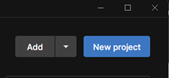
\includegraphics[width=1\textwidth]{NewProject.png}
    \caption{NewProject}
    \label{fig:NewProject}
\end{figure}

Er verschijnt dan een nieuw scherm. Hier kan er gekozen worden wat soort project gemaakt zal worden. Voor deze casus wordt de “2D (Built-In Render Pipeline)” gekozen. Deze staat onder de categorie Core. Je geeft dan de gewenste naam en locatie.

\begin{figure}[H]
    \centering
    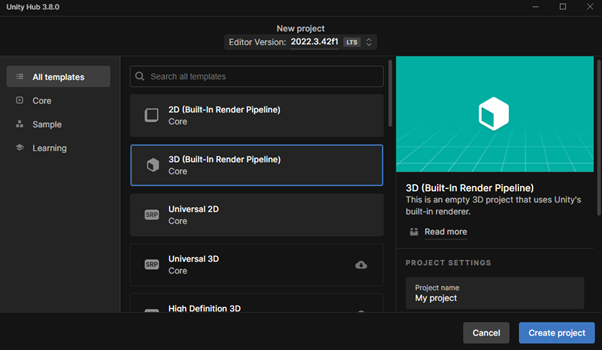
\includegraphics[width=1\textwidth]{Select2D.png}
    \caption{Select2D}
    \label{fig:Select2D}
\end{figure}
Er zijn nog andere mogelijkheden. Sample biedt al gemaakt projecten aan zodat deze als voorbeeld kunnen gebruikt worden. Learning is waar er volledige lessen worden aangeboden om spellen te leren maken.
Nu verschijnt het aangemaakte project in de Unity Hub onder “Projects”.

\begin{figure}[H]
    \centering
    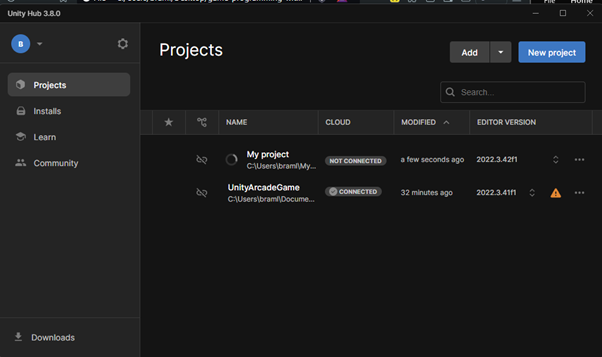
\includegraphics[width=1\textwidth]{Projects.png}
    \caption{Projects}
    \label{fig:Projects}
\end{figure}
Tegerlijkertijd zal je project geopend worden. Dit kan een enige tijd duren.

\subsection{Unity editor}
Eenmaal het project geopend is verschijnt het volgende scherm. Deze is in verschillende schermen onderverdeeld.
\begin{figure}[H]
    \centering
    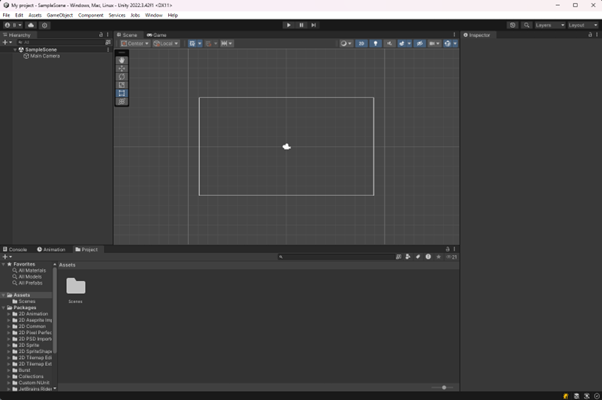
\includegraphics[width=1\textwidth]{UnityEditor.png}
    \caption{UnityEditor}
    \label{fig:UnityEditor}
\end{figure}
Aan de linkerkant bevindt zich de “Hierarchy”. Dit weergeeft wat de huidige scene allemaal bezit.

\subsubsection{Project scherm}
Hierin zijn alle assets terug te vinden die gebruikt worden of zullen gebruikt worden. Voor dit project worden de assets onderverdeeld in de volgende mappen: Scenes, Scripts, Prefabs, Ship en Enemies. Bij het aanmaken van het project is de map Scenes al gemaakt.

\subsubsection{Scene scherm}
Hierin is de omgeving waar het spel plaatsvindt te vinden. Elk level heeft een scene. Scenes worden opgeslagen als assets waardoor de Sample Scene terug te vinden is in de Scenes folder.

Een scene is opgemaakt uit verschillende objecten, deze worden ook gameobjects genoemd. Door gebruik te maken van de scene scherm kan er genavigeerd worden in de scene zonder de scene te moeten builden en renderen.

\subsection{Ship laten bewegen}
In dit onderdeel wordt uitgelegd hoe de speler van het spel een ruimteschip kan laten bewegen. De eerste stap is de afbeelding van het ruimteschip in de in het project te steken. Dit kan via oftewel het in het project scherm te slepen of de map te openen in de explorer en deze daarin te slepen. Eenmaal dit gebeurd is verschijnt de afbeelding in het project en kan deze in de scene geslepen worden.  

\begin{figure}[H]
    \centering
    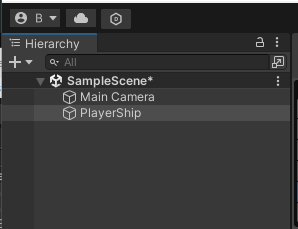
\includegraphics[width=1\textwidth]{SampleSceneImage.png}
    \caption{SampleSceneImage}
    \label{fig:SampleSceneImage}
\end{figure}

De afbeelding van het ship is nog wazig. Dit komt omdat de editor niet goed weet welke soort afbeelding het is. Dit is te verhelpen door op de afbeelding te klikken in het project. Rechts verschijnt er een nieuw scherm genaamd “Inspector”. Hierin kunnen allerlei eigenschappen aangepast worden. Voor dit voorbeeld veranderen er twee zaken. Filter mode moet naar de optie “Point (no filter)” en de optie “Pixels per unit” van 100 naar 32. Dit hangt af van hoe de afbeelding is gemaakt. Voor dit voorbeeld is deze 32 pixels.

\begin{figure}[H]
    \centering
    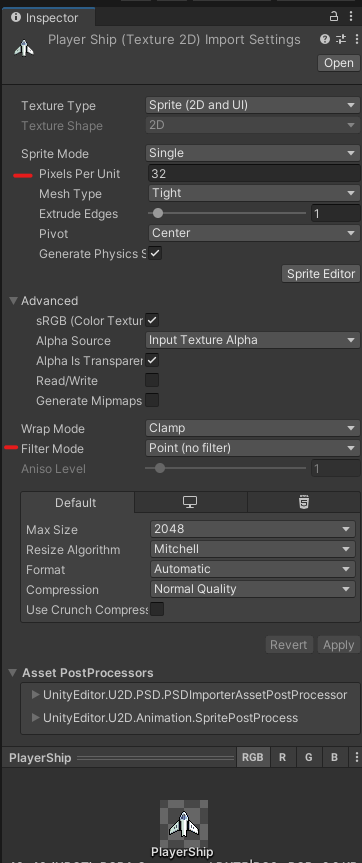
\includegraphics[width=1\textwidth]{PlayerInspector.png}
    \caption{PlayerInspector}
    \label{fig:PlayerInspector}
\end{figure}

Om nu het ship van links naar rechts te doen bewegen bij invoer van de speler moet er een script toegevoegd worden aan de game object. Dit doe je door in de “Hierarchy” het schip aan te duiden. Vervolgens op de knop “Add Component” te klikken en de optie new script selecteren. De naam voor dit script is PlayerController. Eenmaal het script is aangemaakt verschijnt deze in de assets folder in het project. Versleep het naar de folder Scripts zo dat alles overzichtelijk blijft. Het script kan geopend worden door te dubbel klikken op het script.  
In het script zitten er standaard twee functies. De eerste, genaamd Start is waar de logica moet komen die bij het aanmaken van het gameobject moet gebeuren. De tweede functie genaamd Update wordt elke frame van het spel uitgevoerd. De volgende lijnen code zijn nodig om het bewegen van het schip waar te maken. De eerste is om een publiek attribuut aan te maken om zo in de editor de snelheid van het ship te kunnen aanpassen. Eenmaal de snelheid naar wens is kan je deze privaat maken. De volgende lijn code is wat in de Update functie moet staan

\begin{lstlisting}[style=csharp]
    transform.Translate(Vector2.right * MoveSpeed * Time.deltaTime);
\end{lstlisting}

Transform betekend om het object te verplaatsen. Vector2 wordt gebruikt omdat we in een 2D omgeving zitten. De MoveSpeed is voor hoe snel het object moet bewegen en Time.deltaTime zorgt ervoor dat het in seconden verplaats in plaats van elke frame zodat deze soepeler beweegt. In de Input Manager zijn alle invoeren terug te vinden. Deze kan geraadpleegd worden bij “Edit” die vanboven te vinden is. Vervolgens op Project Settings te klikken en bij input manager de map Axes uit te klappen.

\begin{figure}[H]
    \centering
    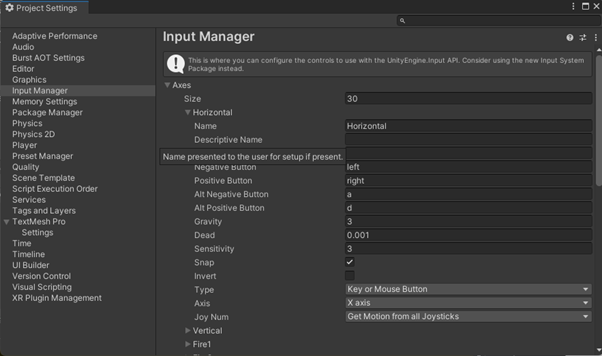
\includegraphics[width=1\textwidth]{InputManager.png}
    \caption{InputManager}
    \label{fig:InputManager}
\end{figure}

Hier is terug te vinden dat de toetsten a en de linkse pijl zijn voor naar links te gaan en d en de rechtse pijl voor naar rechts zijn. Dit kan aangepast worden naar keuze als het systeem bijvoorbeeld een azerty toetsenbord heeft.
Nu dit gekend is kan de invoer van de speler toegevoegd worden aan het script. De invoer wordt opgeslagen in een float. Maak hiervoor een attribuut aan genaamd “HorizontalInput” die als type float heeft. In de update functie wordt deze lijn code bovenaan toegevoegd

\begin{lstlisting}[style=csharp]
    HorizontalInput = Input.GetAxisRaw("Horizontal");
\end{lstlisting}

Deze zorgt ervoor dat bij elke update wordt gekeken welke knop van de Horizontal axis wordt ingedrukt en geeft een waarde terug. Ofwel 1, 0 of -1. Deze waarde wordt nu bij de formule gestoken die eronder staat om zo naar links en naar rechts te gaan. Dit kan nu getest worden doormiddel van op de afspeel knop te klikken in de Unity editor.
Op dit moment kan het schip ook buiten beeld gaan. Dit kan voorkomen worden door grenzen oftewel boundaries toe te voegen. Dit kan door in de Hiërarchie rechtermuisklik te klikken en “Create Empty” te kiezen en het de naam “Left Boundary” te geven. Hierna kan je rechts zaken toevoegen aan dit object. Het eerste dat nodig is is een Box Collider 2D. Je kan deze aanpassen door naast Edit Collider de knop te drukken. Nu kan je deze naar de hoogte van het scherm brengen. De breedte maakt niet uit in dit geval. Er zijn 2 boundaries nodig, een voor links en een voor rechts. Voor een kopie te maken van de reeds gemaakte boundary selecteer deze en doe “crtl+d”. Versleep deze naar de rechtse kant. Deze grenzen moeten een tag krijgen zodat ze op een later moment herkenbaar zijn voor bepaalde scripten. Dit kan door beide Boundary’s aan te duiden en ze de tag Boundary geven. 

\begin{figure}[H]
    \centering
    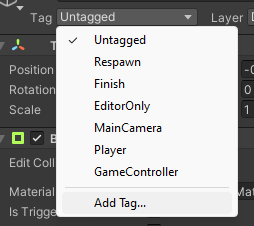
\includegraphics[width=1\textwidth]{AddTag.png}
    \caption{AddTag}
    \label{fig:AddTag}
\end{figure}

Bij het klikken van “Add Tag…” opent er een scherm en kunnen er niet standaard tags toegevoegd worden.

\begin{figure}[H]
    \centering
    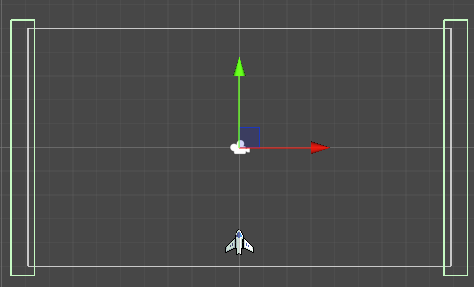
\includegraphics[width=1\textwidth]{Boundaries.png}
    \caption{Boundaries}
    \label{fig:Boundaries}
\end{figure}

Om nu het schip niet door deze grenzen laten gaan moet een “Box Collider 2D” en een”Rigid Body 2D” aan het schip worden toegevoegd. Hierdoor kan het schip niet meer door deze grenzen gaan. Zorg ervoor dat de box collider rond het ship is en dat bij de rigid body de optie “Gravity Scale” op nul staat. Anders zakt het ship naar beneden.
Als laatst stap van dit onderdeel wordt er een achtergrond toegevoegd aan het spel. Dit kan door eenvoudig een afbeelding in het Scene scherm slepen en naar de gewenste grootte af te stellen.

\subsection{Vijanden toevoegen}
In dit onderdeel zal besproken worden hoe je vijanden kan implementeren en ze kan laten bewegen van links naar rechts. Bij elke keer ze het einde van het speelveld bereiken zullen ze zakken en omkeren.
Eerst en vooral moeten de vijanden hun afbeeldingen toegevoegd worden aan het project. In dit geval hebben ze een animatie die afgespeeld zal worden wanneer deze vernietigd worden door de speler. Dit komt in een later onderdeel aanbod maar dit kan nu al klaargezet worden.

\begin{figure}[H]
    \centering
    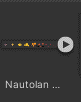
\includegraphics[width=1\textwidth]{AssetAnimated.png}
    \caption{AssetAnimated}
    \label{fig:AssetAnimated}
\end{figure}

Eenmaal ze in het project zitten is te zien dat het als 1 afbeelding wordt beschouwd. Dit moet aangepast worden zodat het als een animatie of een reeks afbeeldingen gezien wordt. Bij het selecteren van de afbeelding kan je de inspector zien van de afbeelding. De optie “Sprite Mode” kan je selecteren wat voor type afbeelding het is. In dit geval duiden we de optie “Multiple” aan. Hierdoor weet de engine dat deze asset uit een reeks van afbeeldingen bestaat. Bij het klikken van sprite editor kan de afbeelding geknipt worden naar een reeks van afbeeldingen. Rechtsboven is de dropdown menu slice te vinden. Hierin kan je aangeven hoe de afbeelding geknipt moet worden. In dit geval bestaat het uit 9 onderdelen. Klik op apply om de veranderingen te bevestigen.

\begin{figure}[H]
    \centering
    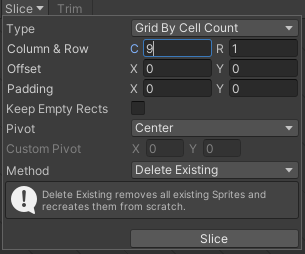
\includegraphics[width=1\textwidth]{SliceSprite.png}
    \caption{SliceSprite}
    \label{fig:SliceSprite}
\end{figure}
Als je nu terugkijkt in de asset folder van enemies kan je de aangepaste afbeelding uit klappen om te zien waaruit ze bestaat.
Om nu de animatie aan te maken en te laten spelen moet dit geconfigureerd worden. Dit kan doormiddel van op het gameobject te klikken van de vijand. Hierna kan je het animation scherm openen. Hierin staan alle animaties die voor het geselecteerd game object bestaan. De eerste animatie is voor als er niets speciaal is oftewel “Idle” genoemd. Bij dit voorbeeld bestaat deze maar uit 1 afbeelding. Je kan deze aanmaken door op de create knop te klikken in het midden van het scherm. 

\begin{figure}[H]
    \centering
    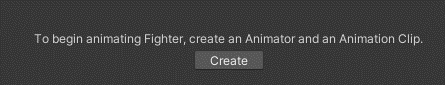
\includegraphics[width=1\textwidth]{CreateAnimationClip.png}
    \caption{CreateAnimationClip}
    \label{fig:CreateAnimationClip}
\end{figure}

Dit krijgt een unieke en herkenbare naam voor een overzicht te behouden. Eenmaal aangemaakt is de animatie links te beheren. Uit het project scherm navigeer naar de afbeelding van het schip zonder de onderverdeling. Sleep deze op de tijdlijn.
Nu is de vernietigings animatie aan de beurt. Eerst moet er een nieuwe animatie aangemaakt worden. Deze krijgt de naam “Destroyed” + om welk type vijand het gaat.
\begin{figure}[H]
    \centering
    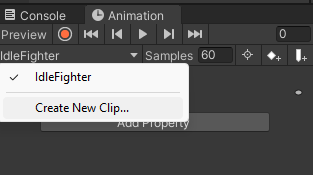
\includegraphics[width=1\textwidth]{NewClip.png}
    \caption{NewClip}
    \label{fig:NewClip}
\end{figure}

Selecteer nu alle afbeelding van de asset die uit meerdere afbeelding bestaat en sleep deze op de tijdlijn. Bij het afspelen van deze animatie zijn twee zaken te zien. De animatie gebeurt redelijk snel en zit vast in een lus. De snelheid kan aangepast worden door bij samples wat standaard de waarde 60 heeft te veranderen naar een lager getal. Voor dit voorbeeld volstaat 12. Om nu de lus ook stop te zetten van het object kan via het detail scherm van de animatie. Deze is terug te vinden door in het project scherm de animatie aan te duiden en rechts de optie “Loop” af te vinken.
Nu dit klaar staat voor een verder onderdeel gaan we verder met het verwezenlijken van de vijanden van links naar rechts en omgekeerd te laten bewegen. Eerst worden de schepen in een overkoepelende map gestoken zodat dit beter bewerkbaar is. Dit kan door een “Empty Object” aan te maken en de schepen erin te slepen.

\begin{figure}[H]
    \centering
    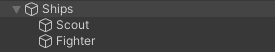
\includegraphics[width=1\textwidth]{Schepen.png}
    \caption{Schepen}
    \label{fig:Schepen}
\end{figure}

Het ships object krijgt nu het script om de schepen te manipuleren en te beheren. Maak hiervoor het script ShipMovement aan en open deze in de code editor. Vooraleer het script geschreven wordt moet de aanraking van de grenzen herkent kunnen worden. Dit moet als volgt. Selecteer het ships game object en voeg een Box Collider 2D toe aan dit object. Verander de vorm van deze box naar de gewenste afmeting startend van het eerste vijandig schip en het laatste. De optie “Is Trigger” moet aangeduid zijn om de functie te laten werken.

\begin{figure}[H]
    \centering
    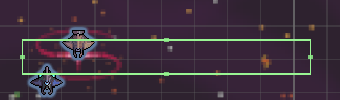
\includegraphics[width=1\textwidth]{BoxShips.png}
    \caption{BoxShips}
    \label{fig:BoxShips}
\end{figure}

Het object heeft ook nog een “Rigidbody 2D” nodig. Als deze is toegevoegd moet er nog wat opties aangepast worden. De gravity scale moet op nul zodat de vijanden niet in een vrijeval belanden. De andere is dat het object niet mag kunnen draaien. Dit kan via de freeze rotation voor de Z as aan te duiden. 

\begin{figure}[H]
    \centering
    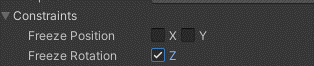
\includegraphics[width=1\textwidth]{FreezeRotation.png}
    \caption{FreezeRotation}
    \label{fig:FreezeRotation}
\end{figure}

Nu dit is gemaakt kan er in het script de logica geschreven worden die ervoor zorgt dat de schepen hun richting veranderen bij de grens. Het script ziet er als volgt uit:

\begin{lstlisting}[style=csharp]
    public class ShipsMovement : MonoBehaviour
    {
        private float MovementSpeed;
        // Start is called before the first frame update
        void Start()
        {
            MovementSpeed = 2;
        }
        
        // Update is called once per frame
        void Update()
        {
            transform.Translate(Vector2.right * MovementSpeed * Time.deltaTime);
        }
        
        private void OnTriggerEnter2D(Collider2D collision)
        {
            if(collision.gameObject.tag == "Boundary")
            {
                transform.position = new Vector3(transform.position.x, transform.position.y - 1, transform.position.z);
                MovementSpeed *= -1;
            }
        }
    }
\end{lstlisting}

\subsection{Speler en vijanden laten schieten}
In dit onderdeel wordt de focus gelegd op het verwezenlijken van dat de speler en de vijanden kunnen schieten. 
De eerste stap is de kogels/projectielen in het project te slepen. Deze kogels kunnen geanimeerd of normaal zijn. Sleep deze in het spel. Dit projectiel krijgt een script genaamd Projectile. Hierin wordt de logica geschreven om de raket te laten bewegen naar boven. Hierin moet deze lijn code in de updatefunctie komen.
\begin{lstlisting}[style=csharp]
    transform.Translate(Vector2.up * 3 * Time.deltaTime);
\end{lstlisting}

Dit game object wordt nu opgeslagen als een prefab. Dit is een soort template waardoor de aanpassing maar 1 keer moeten gebeuren en niet bij alle instanties. Dit kan aangemaakt worden door het game object te verslepen in het project. Er wordt dan automatisch er een prefab van gemaakt.

\begin{figure}[H]
    \centering
    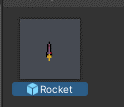
\includegraphics[width=1\textwidth]{Rocket.png}
    \caption{Rocket}
    \label{fig:Rocket}
\end{figure}

Om een speler de mogelijkheid te geven om te schieten moet er een script geschreven worden. Voeg aan het playership object een script toe. Het script bestaat uit volgende onderdelen. Het eerste is dat je een Gameobject moet hebben. In dit geval is dat de kogel die net is gemaakt. Als deze publiek staat kan je in de editor de rocket projectile hierin verslepen. Nu kunnen we deze laten verschijnen elke keer er een aanval knop wordt ingedrukt. Deze is terug te vinden in de input manager. Standaard is dit muis 1 of spacebar.

\begin{lstlisting}[style=csharp]
    void Update()
    {
        if (Input.GetButtonDown("Fire1"))
        {
            Instantiate(projectilePrefab, transform.position, Quaternion.identity);
        }
    }
\end{lstlisting}
Nu is het mogelijk om als speler te schieten. Het volgende is dat de vijanden vernietigd worden bij aanraking van de speler hun shot. Hiervoor wordt er weer gebruik gemaakt van de OnTriggerEnter2D functie. Hiervoor moeten de enemies de tag hun unieke tags krijgen. In dit geval is er een scout ship en een fighter ship. Dit is nodig zodat de juiste animatie kan gespeeld worden. Het projectiel ontbreekt ook nog een Box Collider 2D. Vink bij dit ook de optie Is Trigger aan. De vijanden moeten ook nog elk een box collider krijgen. Hierdoor kan het herkent worden door de engine. Eenmaal dit is gebeurt kan de logica geschreven worden in het script. Hierbij wordt de functionaliteit van dat eenmaal een ship vernietigd word de animatie moet spelen.
Iets dat opmerkelijk is dat eenmaal de speler shit de projectielen voor altijd blijven bestaan als de speler mist. Dit kan opgelost worden door een nieuwe boundary toe te voegen aan de bovenkant.

\begin{lstlisting}[style=csharp]
    private void OnTriggerEnter2D(Collider2D collision)
    {
        if (collision.gameObject.CompareTag("Fighter") || collision.gameObject.CompareTag("Scout"))
        {
            Animator enemyAnimator = collision.gameObject.GetComponent<Animator>();
            if (enemyAnimator != null)
            {
                if (collision.gameObject.CompareTag("Fighter"))
                {
                    enemyAnimator.Play("DestroyedFighter");
                }
                else if (collision.gameObject.CompareTag("Scout"))
                {
                    enemyAnimator.Play("DestroyedScout");
                }
                
                Destroy(collision.gameObject, enemyAnimator.GetCurrentAnimatorStateInfo(0).length + 0.75f);
            }
            else
            {
                Destroy(collision.gameObject); // If no animator, destroy immediately
            }
            
            Destroy(gameObject); // Destroy the current gameObject (the one this script is attached to)
        }
        else if (collision.gameObject.CompareTag("Boundary"))
        {
            Destroy(gameObject);
        }
    }
\end{lstlisting}

\subsection{Levens implementeren}
In dit onderdeel wordt de user interface gemaakt en kan de speler levens verliezen wanneer deze geraakt wordt door de vijand.
De eerste stap is het aanmaken van de user interface. Dit kan door in de hierarchie rechtermuisklik te doen en onder ui image te selecteren. Wat meteen opvalt is dat dit vele malen groter is dan al de rest. Dit is normaal. Als het spel gestart wordt kan er waargenomen worden dat dit op zijn plek valt. Bij de image kan je de source aanpassen naar de gewenste afbeelding. Hiervoor wordt in dit geval de speler zijn afbeelding gebruikt. Deze worden nu gedupliceerd naar de hoeveelheid levens er gewenst zijn.
Om een tekst toe te voegen aan de ui wordt er gebruik gemaakt van textmeshpro. Bij de eerste keer dit te gebruiken verschijnt er een popup met de vraag om TMP te importeren. Dit is nodig om TMP te kunnen gebruiken. Eenmaal de import is afgerond kan er gebruikt gemaakt worden van text.
Om de levens te beheren is een nieuw script nodig. Deze krijgt de naam LivesManager. Dit script wordt verbonden met de speler zijn ship. Een speler start in dit geval met 3 levens. Dit wordt opgeslagen in een integer. Maak deze publiek zodat je in de editor deze kan aanpassen. De speler kan levens verliezen op verschillende manieren. De eerste is als de speler in contact komt met een vijandig schip. Hiervoor wordt gebruik gemaakt van de functie OnCollisionEnter2D. Deze functie start telkens de speler in aanraking komt met een ander object. Voor dit geval is het alleen nodig wanneer deze in aanraking komt met een vijandig schip. Dit kan doormiddel van een if clausule die kijkt naar welke tag het object heeft. In dit geval “Scout” of “Fighter”.  Als dit gebeurt wordt het aantal levens verminderd en wordt de vijand verwijderd. Eenmaal de speler al hun levens kwijt is wordt de speler hun ship verwijderd. 
Om ervoor te zorgen dat het aantal levens in ui worden aangepast moet in het script een lijst van Image komen om zo ervoor te zorgen dat bij elk leven dat verloren gaat er een afbeelding verdwijnt. De code ziet er als volgt uit:

\begin{lstlisting}[style=csharp]
    public class PlayerLives : MonoBehaviour
    {
        public int lives = 3;
        public Image[] livesUi;
        
        public PointManager pointManager;
        public GameManager gameManager;
        // Start is called before the first frame update
        void Start()
        {
            
        }
        
        // Update is called once per frame
        void Update()
        {
            
        }
        
        private void OnCollisionEnter2D(Collision2D collision)
        {
            if (collision.collider.gameObject.CompareTag("Fighter") || collision.collider.gameObject.CompareTag("Scout"))
            {
                Destroy(collision.collider.gameObject);
                lives -= 1;
                for (int i = 0; i < livesUi.Length; i++){
                    if(i < lives)
                    {
                        livesUi[i].enabled = true;
                    }
                    else
                    {
                        livesUi[i].enabled = false;
                    }
                }
                if(lives <= 0)
                {
                    Destroy(gameObject);
                }
            }
        }
    }
    
\end{lstlisting}
Nu dit gebeurd is kunnen we in de ui de eerder gemaakte en geplaatste afbeeldingen in deze lijst slepen. In onderstaande afbeelding is hoe het eruit moet zien.

\begin{figure}[H]
    \centering
    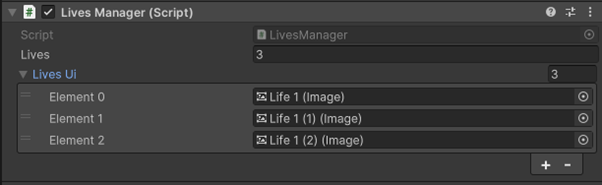
\includegraphics[width=1\textwidth]{LivesManager.png}
    \caption{LivesManager}
    \label{fig:LivesManager}
\end{figure}

\subsection{Score}
Om score te implementeren hebben moet er eerst een tekstveld worden toegevoegd aan de user interface. Dit kan door rechtermuisklik op Canvas en onder ui tekst te selecteren. De tekst die erin komt te staan is “Score: 9999”. Dit is een placeholder. Nu gaan we het script maken die dit kan aanpassen. Het script hoort bij een leeg gameobject genaamd PointManager. Eenmaal deze is gemaakt kan het script geopent worden. Deze bezit twee attributen. Een voor het textveld met het type  “TMP_Text” en een andere voor de score met type integer. In de al reeds gemaakte Start functie zetten we de score op nul en veranderen we de tekst naar “Score: “ + score. Hierdoor zal bij opstart van het spel initieel op 0 te komen staan. Voor het verhogen van de punten wordt een nieuwe publieke functie aangemaakt genaamd UpdateScore(int points). Hierdoor kunnen er in andere scripts die de Pointmanager bezitten deze functie aanroepen. Om dit te laten werken moeten we het script Projectile aanpassingen aanbrengen. Eerst en vooral moet er een extra property voor PointManager toegevoegd worden aan het script. Hierna komt er logica bij de funtie OntriggerEnter2D. Bij het raken van een vijand wordt de pointmanager de functie UpdateScore op geroepen met hoeveel punten gewenst.

\begin{lstlisting}[style=csharp]
    public class Projectile : MonoBehaviour
    {
        public float moveSpeed = 2;
        private PointManager pointManager;
        // Start is called before the first frame update
        void Start()
        {
            pointManager = GameObject.Find("PointManager").GetComponent<PointManager>();
        }
        
        // Update is called once per frame
        void Update()
        {
            transform.Translate(Vector2.up * moveSpeed * Time.deltaTime);
        }
        private void OnTriggerEnter2D(Collider2D collision)
        {
            if (collision.gameObject.CompareTag("Fighter") || collision.gameObject.CompareTag("Scout"))
            {
                Animator enemyAnimator = collision.gameObject.GetComponent<Animator>();
                if (enemyAnimator != null)
                {
                    if (collision.gameObject.CompareTag("Fighter"))
                    {
                        enemyAnimator.Play("DestroyFighter");
                        pointManager.UpdateScore(100);
                    }
                    else if (collision.gameObject.CompareTag("Scout"))
                    {
                        enemyAnimator.Play("DestroyScout");
                        pointManager.UpdateScore(50);
                    }
                    
                    Destroy(collision.gameObject, enemyAnimator.GetCurrentAnimatorStateInfo(0).length + 0.75f);
                }
                else
                {
                    Destroy(collision.gameObject); // If no animator, destroy immediately
                }
                
                Destroy(gameObject); // Destroy the current gameObject (the one this script is attached to)
            }
            else if (collision.gameObject.CompareTag("Boundary"))
            {
                Destroy(gameObject);
            }
        }
\end{lstlisting}
\subsection{Einde spel}
Het spel moet kunnen eindigen. Dit gebeurt wanneer de speler al hun levens verloren heeft. Om dit te kunnen realiseren is er nood aan een GameManager. Deze kan de status van de game beheren en zo bij het einde van het spel het spel stoppen en laten herstarten. De Gamemanager bestaat uit een leeg object met een script zoals de PointManager van het vorig onderdeel. Voor dat het script geschreven wordt moet er een scherm gemaakt worden die over het spel getoond wordt bij het einde van het spel. In het canvas waar de elementen zitten voor de levens te tonen komt er een nieuw panel. Voeg deze toe aan het canvas en geeft het de naam GameOverPanel. Hierin komen de volgende zaken in terecht. Eerst een tekstveld voor Game Over te tonen. Hieronder komt links de highscore de speler behaald heeft en rechts de score van het huidig spel. Deze bestaan telkens uit twee tekstvelden. Een voor de tekst zelf en een ander voor de score. Deze zijn gescheiden omdat de Pointmanager deze dan zou kunnen aanvullen bij het einde van het spel. Onderaan komt er nog een knop om het spel te herstarten. Het scherm ziet er als volgt uit:

\begin{figure}[H]
    \centering
    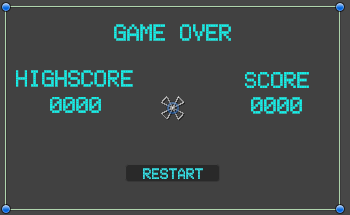
\includegraphics[width=1\textwidth]{GameOverScreen.png}
    \caption{GameOverScreen}
    \label{fig:GameOverScreen}
\end{figure}

Dit scherm moet standaard niet geactiveerd zijn. Dit kan door op GameOverPanel te klikken en rechts in de inspector het vinkje bovenaan af te vinken.
In het script van de gamemanager moeten er 3 functies geschreven worden. De eerste is om het spel te doen stoppen en het GameOverPanel te laten tonen. 

\begin{lstlisting}[style=csharp]
        public void GameOver()
    {
        Time.timeScale = 0;
        gameOverPanel.SetActive(true);
    }
\end{lstlisting}

Een tweede functie om het spel te laten herstarten. Dit gebeurt door de time.scale weer op 1 te zetten en de  scene manager de scene opnieuw te laten lopen.
\begin{lstlisting}[style=csharp]
    public void Restart()
    {
        Time.timeScale = 1;
        SceneManager.LoadScene(SceneManager.GetActiveScene().buildIndex);
    }
    
\end{lstlisting}

De GameOver functie wordt aangesproken in de LivesManager functie. Bij de if clausules waar de levens gelijk of kleiner dan 0 te komen te staan moet de GameManager.GameOver() aangeroepen worden. Hierdoor weet het spel dat het gestopt moet worden bij het verlies van alle levens. 
De restart functie behoort tot de restart knop die bij het GameOverPanel zit. Bij het selecteren van de knop is onderaan te zien dat er een functie kan aangewezen worden. Sleep de GameManager hierin en selecteer de juist functie genaamd GameOver.

\begin{figure}[H]
    \centering
    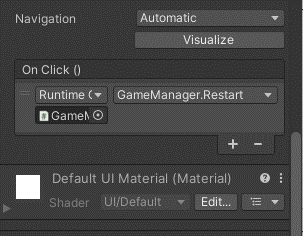
\includegraphics[width=1\textwidth]{RestartFunctie.png}
    \caption{RestartFunctie}
    \label{fig:RestartFunctie}
\end{figure}

\subsection{ Exporteren van het spel}
Nu het spel is afgewerkt is het klaar om het te exporteren naar een executeable zodat het spel op verschillende systemen gespeeld kan worden. 
Navigeer naar File dat rechtsboven staat. Klik op Build Settings… De shortcut voor dit is crtl+shift+B. Eenmaal dit is geopend selecteer het juiste platform. In dit geval is dit Windows, Mac, Linux. Rechts kan dan het Target Platform geselecteerd worden. In dit geval Windows. Klik nu onderaan op switch platform. Hierna slepen we alle scenes die nodig zijn om het spel te runnen in het Scenes in Build vak. De eerste scene in dit vak is ook de start scene. Hoe hier rekening mee.
Voordat op build gedrukt wordt kunnen er nog player settings aangepast worden. Hierin kan het icoon dat het spel krijgt gekozen worden en welke resolutie het spel gespeeld moet worden.

\begin{figure}[H]
    \centering
    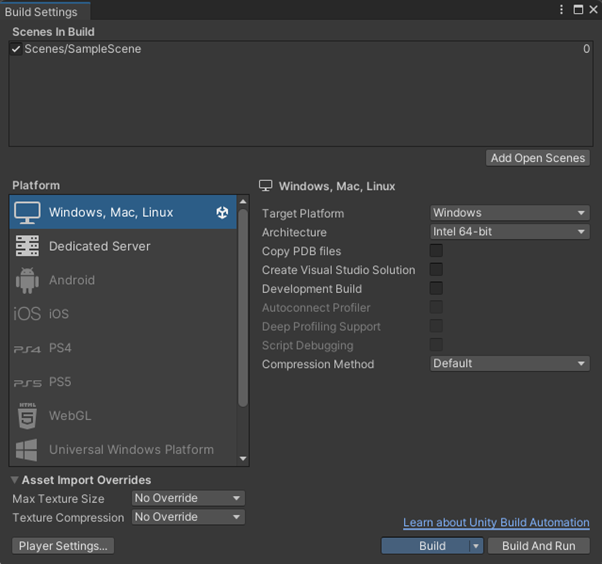
\includegraphics[width=1\textwidth]{BuildScherm.png}
    \caption{BuildScherm}
    \label{fig:BuildScherm}
\end{figure}
Eenmaal dit allemaal gekozen is kan het spel gebuild worden. Dit opent de file explorer om een locatie te selecteren waar het spel gemaakt mag worden. Het is aangeraden om dit op te slaan in een lege map op een locatie naar keuze. Voor dit voorbeeld komt deze op het bureaublad. Als het spel heeft alles wat in deze map terecht komt nodig om het spel te kunnen spelen.
\subsection{Eindresultaat}
Het eindresultaat is te zien aan de onderstaande foto. De github repository is te vinden via deze link: \url{https://github.com/BramLippens/UnityArcadeGame}
\begin{figure}[H]
    \centering
    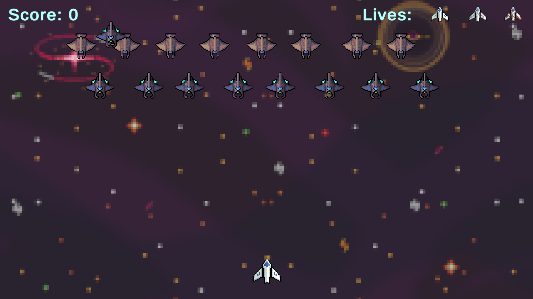
\includegraphics[width=1\textwidth]{UnityGameFinished.png}
    \caption{UnityGameFinished}
    \label{fig:UnityGameFinished}
\end{figure}
\section{Implementatie Godot}
Het spel is ontwikkeld in de Godot-engine met behulp van de programmeertaal C\#. Om aan de slag te gaan, dient u eerst de Godot-engine te downloaden van de officiële website. Er zijn twee verschillende versies beschikbaar. De standaardversie is geschikt indien u gebruik wilt maken van de ingebouwde scripttaal GDScript, een functionele programmeertaal. De alternatieve versie biedt ondersteuning voor C\#.
\\
Na het downloaden en uitpakken van de engine zijn er geen verdere installatiestappen vereist, in tegenstelling tot sommige andere engines. Bij het openen van Godot worden verschillende panelen gepresenteerd.
\\
Bij het aanmaken van een nieuw project in Godot kan men kiezen uit drie verschillende renderers. De eerste, genaamd "Compatibility", is geschikt voor eenvoudige 2D-videospellen en biedt betere speelbaarheid op oudere apparaten. Deze renderer maakt gebruik van OpenGL 3 als backend en heeft minder geavanceerde 3D-graphics, wat voor de huidige usecase geen belemmering vormt aangezien er een 2D-spel wordt ontwikkeld.
\\
De tweede renderer, "Mobile", is ontworpen voor de ontwikkeling van videogames voor mobiele apparaten en desktops. Deze biedt verbeterde rendering voor eenvoudigere spellen, vergelijkbaar met de "Compatibility"-renderer. Een nadeel is dat complexere scènes minder schaalbaar zijn met deze renderer.
\\
De derde en laatste optie, "Forward+", is uitsluitend geschikt voor desktop-platformen en is bedoeld voor de ontwikkeling van 3D-videospellen. Deze renderer is geschikt voor het creëren van complexe spellen.

Gezien de specifieke usecase is de "Mobile"-renderer geselecteerd voor de implementatie van het spel.
\\
Na het creëren van een nieuw project wordt het bovenstaande scherm gepresenteerd. Dit scherm bestaat uit verschillende panelen, elk met een specifieke functie. Aan de rechterzijde bevindt zich het scènepaneel, waarin alle nodes worden weergegeven die zich in de huidige scène bevinden. Daaronder is het assets-paneel te vinden, waar alle grafische elementen, zoals afbeeldingen en sprites, worden opgeslagen. Een node kan worden opgeslagen als een scène, waardoor deze herbruikbaar wordt en in het assets-paneel verschijnt. Aan de rechterzijde van het scherm worden de eigenschappen van de momenteel geselecteerde node getoond.
\subsection{Installatie van Godot}
Godot heeft geen installatie nodig. Dit is voorverpakt in een zip bestand. De gebruiker van de engine moet alleen maar deze uitpakken en de engine is klaar om te gebruiken. De download voor de engine is terug te vinden op de volgende link: “https://godotengine.org/download/windows/”.
\begin{figure}[H]
    \centering
    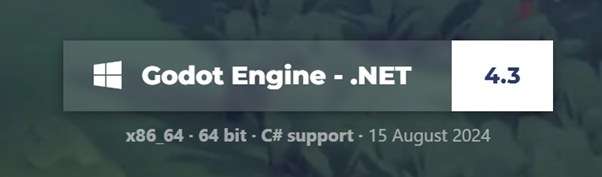
\includegraphics[width=1\textwidth]{GodotDownload.png}
    \caption{GodotDownload}
    \label{fig:GodotDownload}
\end{figure}

Om een nieuw project te starten moet je de .exe van de uitgepakte download runnen. Hiermee opent het scherm “Project Manager”. Klik hierna op create om een project aan te maken. Hierin moet de naam van het project, de plaats waar het opgeslagen moet worden en welke renderer er gebruikt moet worden gekozen. Er zijn 3 verschillende opties voor de renderer. De eerste is Forward+. Deze is voor het ontwikkelen van 3D spellen en grote complexere spellen. Voor deze casus is dit overbodig. Hierdoor wordt er gekozen om de Mobile optie. Deze werkt sneller voor simpele scenes.

\begin{figure}[H]
    \centering
    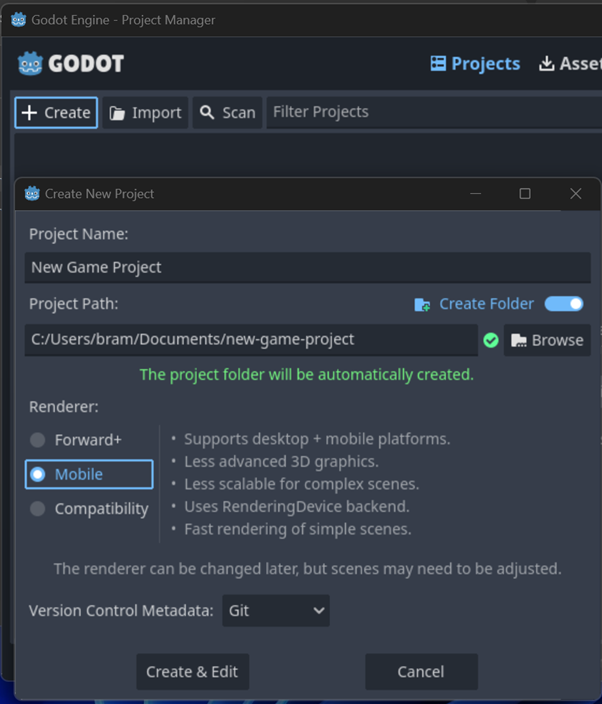
\includegraphics[width=1\textwidth]{CreateGodot.png}
    \caption{CreateGodot}
    \label{fig:CreateGodot}
\end{figure}

\subsubsection{De Godot editor}
Nu het project is aangemaakt opent de editor. Deze is hieronder te zien.
\begin{figure}[H]
    \centering
    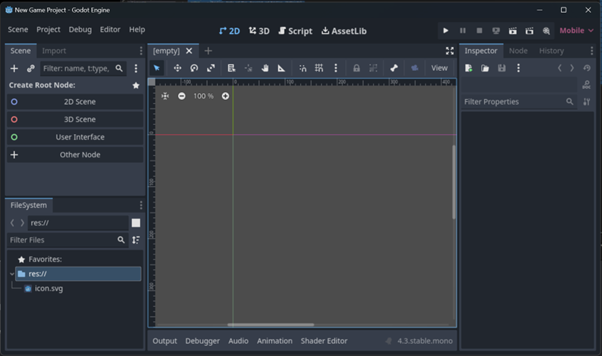
\includegraphics[width=1\textwidth]{GodotEditor.png}
    \caption{GodotEditor}
    \label{fig:GodotEditor}
\end{figure}
Deze is onderverdeeld in verschillende schermen. Links is te zien welke nodes er gebuikt worden. Omdat in een nieuw project er nog niets van nodes zijn aangemaakt is er de optie om de initieel node aan te maken. Hieronder is alles wat in het project gebruikt wordt terug te vinden. Dit kan van assets tot herbruikbare nodes. Aan de rechterzijde is de inspector te vinden. Bij het selecteren van een node of sprite in de scene manager wordt deze aangevuld met allemaal informatie van het geselecteerde item.

\subsection{Speler maken}
Het startpunt voor het maken van de speler is bij een Area2D. Hierin komen de volgende zaken. De sprite2D is een node om een afbeelding toe te voegen aan het object. Deze moet ook een collision2D krijgen. Dit is nodig om als de vijand schiet het te herkennen. De vorm van de collision moet even groot worden als de afbeelding. Nu dit klaar staat krijgt de sprite een script. Dit kan door op het icoontje naast filter zoekbalk te klikken. Bij het aanmaken van het script moet er gekozen worden om C\# te gebruiken.
\begin{figure}[H]
    \centering
    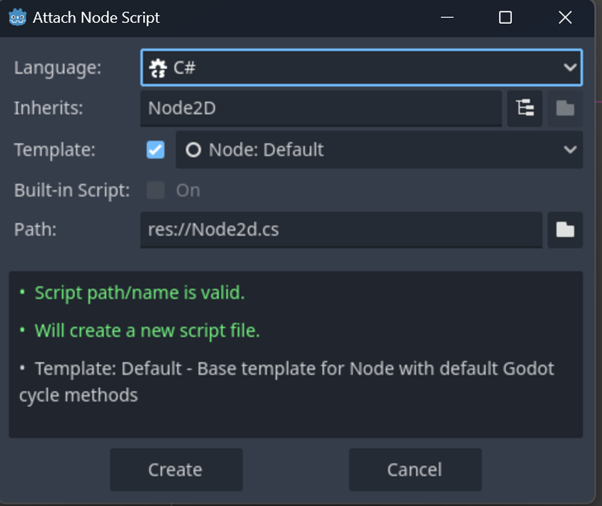
\includegraphics[width=1\textwidth]{GodotScriptMaken.png}
    \caption{GodotScriptMaken}
    \label{fig:GodotScriptMaken}
\end{figure}
In dit script zijn volgende zaken toegevoegd. De snelheid met het type float. Een richting met het type Vector2 omdat het een 2d spel is.  Het script moet ook een reverence hebben naar de collisionshape. Voor de speler te laten bewegen moet er ook de keybindings geconfigureerd worden. Dit is te vinden project -> projectsettings-> input Map. De volgende inputs moeten geconfigureerd worden. “move_left” om naar links te gaan, “move_right” om naar rechts te gaan en “shoot” om te kunnen schieten. Deze hebben we in een later stadia nodig.

\begin{figure}[H]
    \centering
    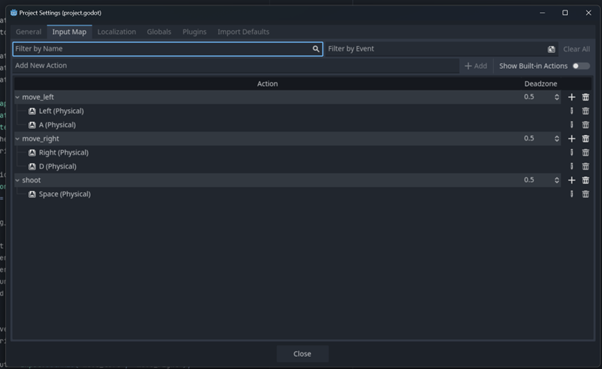
\includegraphics[width=1\textwidth]{MovementSettingsGodot.png}
    \caption{MovementSettingsGodot}
    \label{fig:MovementSettingsGodot}
\end{figure}
Voor dit te laten werken is de volgende functie nodig. Deze kijkt welke input er gegeven wordt laat het schip verschuiven naar de gewenste richting.

\begin{lstlisting}[style=csharp]
    // Called every frame. 'delta' is the elapsed time since the previous frame.
    public override void _Process(double delta)
    {
        var input = Input.GetAxis("move_left", "move_right");
        
        direction = input > 0 ? Vector2.Right : input < 0 ? Vector2.Left : Vector2.Zero;
        
        var deltaMovement = Speed * direction.X * delta;
        if (Position.X + deltaMovement < startBound || Position.X + deltaMovement + bounding_size_x > endBound)
        {
            return;
        }
        
        Position +=  new Vector2((float)deltaMovement, 0);
    }    
\end{lstlisting}

\subsection{De speler laten schieten}
Voor de laser die geschoten wordt te creëren is een nieuwe scene nodig. Het startpunt is een area2d. Hierin komt een sprite2d. Dit is de afbeelding van de laser. De laser moet ook nog een CollisionShape2d krijgen die dezelfde grootte heeft als de afbeelding. Hierna kan het script voor de laser gemaakt worden. Dit script is redelijk eenvoudig. De laser zal constant naar boven.
\begin{lstlisting}[style=csharp]
    using Godot;
    using System;
    
    public partial class Laser : Area2D
    {
        [Export]
        private float Speed = 300;
        // Called when the node enters the scene tree for the first time.
        public override void _Ready()
        {
        }
        
        // Called every frame. 'delta' is the elapsed time since the previous frame.
        public override void _Process(double delta)
        {
            Position -= new Vector2(0, Speed * (float)delta);
        }
    }    
\end{lstlisting}

Om nu de speler te laten schieten moet bij de speler node een extra node toegevoegd worden. Dit wordt het punt vanwaar de laser geschoten wordt. Om dit te laten werken krijgt dit startpunt zijn eigen script. Dit zorgt ervoor dat het overzichtelijk blijft bij het ontwikkelingsproces. Bij elke keer het shoot keybind ingedrukt wordt de laser afgeschoten. Er is in dit voorbeeld ervoor gekozen om maar 1 laser per keer op het scherm te hebben.

\begin{lstlisting}[style=csharp]
    using Godot;
    using System;
    
    public partial class Shooting : Node2D
    {
        [Export]
        PackedScene laserScene;
        
        private Laser currentLaser = null;
        
        public override void _Input(InputEvent @event)
        {
            base._Input(@event);
            
            if(Input.IsActionJustPressed("shoot")){
                if(currentLaser == null){
                    currentLaser = laserScene.Instantiate() as Laser;
                    currentLaser.GlobalPosition = ((Node2D)GetParent()).GlobalPosition - new Vector2(0, 20);
                    GetTree().Root.GetNode<Node>("Main").AddChild(currentLaser);
                    currentLaser.Connect("tree_exited", new Callable(this, nameof(OnLaserExitedTree)));
                }
            }
        }
        public void OnLaserExitedTree()
        {
            currentLaser = null;
        }
    }   
\end{lstlisting}
Wat op te merken is dat de laser blijft bestaan. Dit is niet de bedoeling. Moest dit niet afgehandeld worden kan het performantie problemen veroorzaken. Dit kan verholpen worden door een nieuwe scene aan te maken en deze bovenaan in het speel veld te plaatsen. Deze bestaat uit een CollisionShape2D. Om dit te laten werken is een klein script nodig.
\begin{figure}[H]
    \centering
    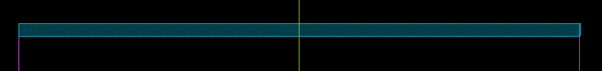
\includegraphics[width=1\textwidth]{LaserCatcher.png}
    \caption{LaserCatcher}
    \label{fig:LaserCatcher}
\end{figure}
Bij het klikken van de laserCatcher is rechts te de eigenschap Collision terug te vinden. Hiermee kan je allerlei zaken configureren zodat deze alleen met laser te laten werken. Om lagen toe te voegen moet er op de drie verticale punten gedrukt worden. Dit opent een nieuw scherm dat alle lagen weergeeft. In layer 2 voer je laser in en vink deze aan in de inspector on mask.
\begin{figure}[H]
    \centering
    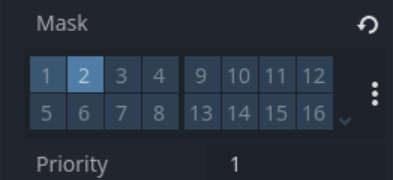
\includegraphics[width=1\textwidth]{MaskGodot.png}
    \caption{MaskGodot}
    \label{fig:MaskGodot}
\end{figure}
Hierdoor is er maar 1 lijntje code nodig bij het script van de laser catcher. Hierdoor worden dus de laser verwijderd bij het einde van het speelveld.

\begin{lstlisting}[style=csharp]
   using Godot;
   using System;
   
   public partial class LaserCatcher : Area2D
   {
       public void OnAreaEntered(Area2D area)
       {
           area.QueueFree();
       }
   }
   
\end{lstlisting}

\subsubsection{Vijanden laten spawnen}
Om vijanden te kunnen laten verschijnen moet er eerst en vooral een startpunt geconfigureerd worden voor dit. Dit gebeurt met behulp van een node die als startpunt gebruikt wordt. 
Voor de vijanden aan te maken is hetzelfde principe als de speler aan te maken. Eenmaal deze zijn aangemaakt kunnen we deze aanroepen in de spawner zodat deze in het spel komen te staan. Dit is het script van hoe dit in zijn werk gaat.
\begin{lstlisting}[style=csharp]
using Godot;
using System;
using System.Collections.Generic;
using System.Linq;

public partial class InvaderSpawner : Node2D
{
    const int ROWS = 5;
    const int COLUMNS = 11;
    const int HORIZONTAL_SPACING = 32;
    const int VERTICAL_SPACING = 32;
    const int INVADER_HEIGHT = 24;
    const int START_Y_POSITION = -50;
    const int INVADERS_POSITION_X_INCREMENT = 10;
    const int INVADERS_POSITION_Y_INCREMENT = 20;
    
    int movement_direction = 1;
    
    public PackedScene InvaderScene { get; set; }
    
    public PackedScene InvaderShotScene { get; set; }
    public Timer MovementTimer { get; set; }
    public Timer ShotTimer { get; set; }
    
    // Called when the node enters the scene tree for the first time.
    public override void _Ready()
    {
        InvaderConfig invader1Res = ResourceLoader.Load("res://Resources/Invader1.tres") as InvaderConfig;
        InvaderConfig invader2Res = ResourceLoader.Load("res://Resources/Invader2.tres") as InvaderConfig;
        InvaderConfig invader3Res = ResourceLoader.Load("res://Resources/Invader3.tres") as InvaderConfig;
        InvaderScene = GD.Load<PackedScene>("res://Scenes/Invader/Invader.tscn");
        InvaderShotScene = GD.Load<PackedScene>("res://Scenes/Invader/InvaderShot.tscn");
        MovementTimer = GetNode<Timer>("MovementTimer");
        MovementTimer.Connect("timeout", new Callable(this,nameof(MoveInvaders)));
        
        ShotTimer = GetNode<Timer>("ShotTimer");
        ShotTimer.Connect("timeout", new Callable(this, nameof(OnInvaderShot)));
        
        
        InvaderConfig invaderConfig;
        for(int row = 0; row < ROWS; row++)
        {
            if (row == 0 || row == 1)
            {
                invaderConfig = invader1Res;
            }
            else if (row == 2 || row == 3)
            
            {
                invaderConfig = invader2Res;
            }
            else
            {
                invaderConfig = invader3Res;
            }
            
            var rowWidth = (COLUMNS * invaderConfig.Width * 3) + (COLUMNS - 1) * HORIZONTAL_SPACING;
            var startX = (Position.X - rowWidth) / 2;
            
            for (int column = 0; column < COLUMNS - 1; column++)
            {
                var x = startX + (column * invaderConfig.Width * 3) + (column * HORIZONTAL_SPACING);
                var y = START_Y_POSITION + (row * INVADER_HEIGHT) + (row * VERTICAL_SPACING);
                var spawnPosition = new Vector2(x, y);
                
                SpawnInvader(invaderConfig, spawnPosition);
            }
        }
    }
    
    private void MoveInvaders()
    {
        Position = Position with { X = Position.X + (movement_direction * INVADERS_POSITION_X_INCREMENT) };
    }
    
    private void SpawnInvader(InvaderConfig invaderConfig, Vector2 spawnPosition)
    {
        // REMBER
        Invader invader = InvaderScene.Instantiate() as Invader;
        
        invader.Config = invaderConfig;
        invader.GlobalPosition = spawnPosition;
        AddChild(invader);
    }
    
    public void OnRightWallAreaEntered(Area2D area)
    {
        if (movement_direction == 1)
        {
            Position = Position with { Y = Position.Y + INVADERS_POSITION_Y_INCREMENT };
            movement_direction = -1;
        }
    }
    public void OnLeftWallAreaEntered(Area2D area)
    {
        if (movement_direction == -1)
        {
            Position = Position with { Y = Position.Y + INVADERS_POSITION_Y_INCREMENT };
            movement_direction = 1;
        }
    }
    public void OnBottomWallAreaEntered(Area2D area)
    {
        GD.Print("Right Wall");
    }
    
    public void OnInvaderShot()
    {
        List<Invader> invaders = GetChildren().Where(x => x is Invader).Cast<Invader>().ToList();
        // get random invader
        Invader randomInvader = invaders[GD.RandRange(0, invaders.Count)-1];
        
        var invaderShot = InvaderShotScene.Instantiate() as InvaderShot;
        invaderShot.GlobalPosition = randomInvader.GlobalPosition;
        
        GetTree().Root.AddChild(invaderShot);
    }
}

\end{lstlisting}
Om de vijand te laten verdwijnen eenmaal deze beschoten wordt kan dit via een extra functie te schrijven bij de vijand hun script. Dit is de onAreaEntered(Area2D area). Deze kan herkennen of het een laser is dat in contact kwam met het schip of niet. Is dit zo dan wordt de vijand verwijderd.
\subsection{Eindresultaat}
Het eindresultaat is te zien aan de onderstaande foto. De github repository is te vinden via deze link: \url{https://github.com/BramLippens/Godot-CSharp-Space-Invaders}
\begin{figure}[H]
    \centering
    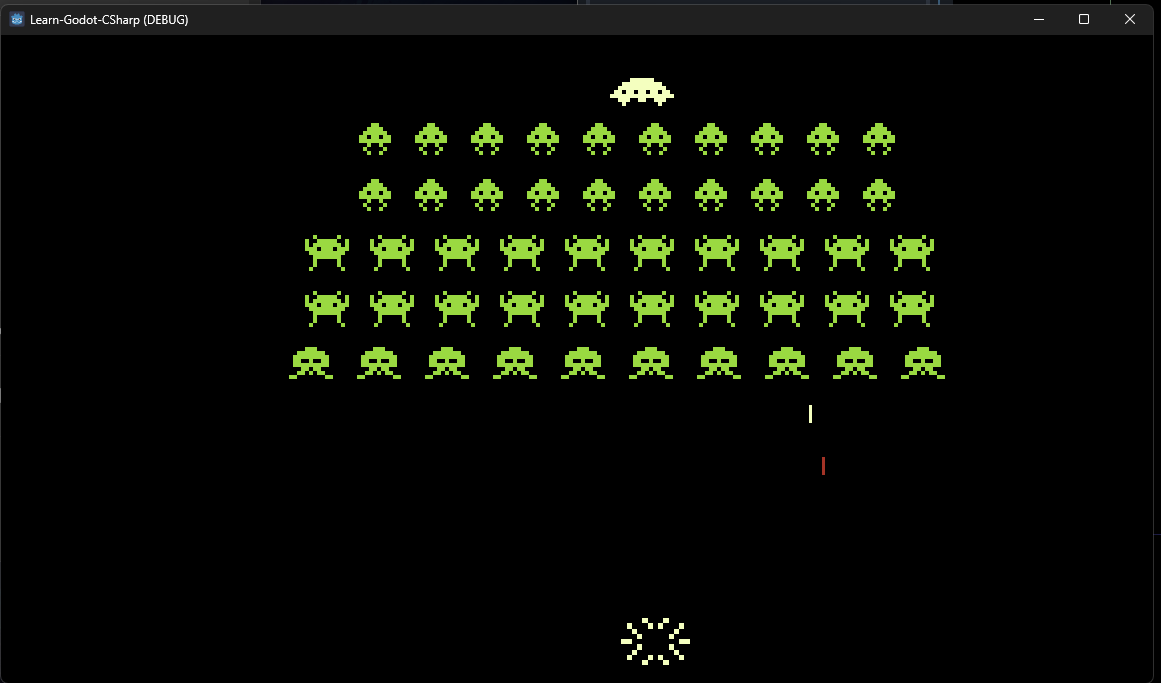
\includegraphics[width=1\textwidth]{ImplementatieSpel.png}
    \caption{Implementatie}
    \label{fig:POC}
\end{figure}

